

\tikzset{every picture/.style={line width=0.75pt}} %set default line width to 0.75pt        

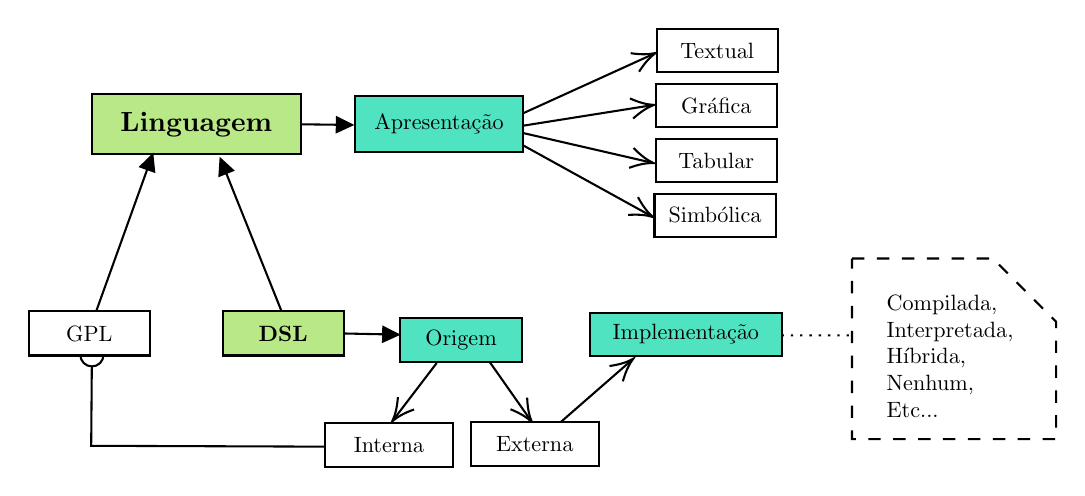
\begin{tikzpicture}[x=0.75pt,y=0.75pt,yscale=-1,xscale=1]
%uncomment if require: \path (0,408); %set diagram left start at 0, and has height of 408

%Shape: Rectangle [id:dp5982497232353539] 
\draw  [fill={rgb, 255:red, 184; green, 233; blue, 134 }  ,fill opacity=1 ] (43.96,49.84) -- (144.49,49.84) -- (144.49,78.83) -- (43.96,78.83) -- cycle ;
%Shape: Rectangle [id:dp8004700532925917] 
\draw  [fill={rgb, 255:red, 255; green, 255; blue, 255 }  ,fill opacity=1 ] (13.5,154.48) -- (71.89,154.48) -- (71.89,175.74) -- (13.5,175.74) -- cycle ;
%Shape: Rectangle [id:dp6645135942832383] 
\draw  [fill={rgb, 255:red, 184; green, 233; blue, 134 }  ,fill opacity=1 ] (106.92,154.48) -- (165.31,154.48) -- (165.31,175.74) -- (106.92,175.74) -- cycle ;
%Straight Lines [id:da940322594025554] 
\draw [fill={rgb, 255:red, 255; green, 255; blue, 255 }  ,fill opacity=1 ]   (45.99,154.48) -- (72.82,79.88) ;
\draw [shift={(73.5,78)}, rotate = 469.78] [fill={rgb, 255:red, 0; green, 0; blue, 0 }  ][line width=0.75]  [draw opacity=0] (8.93,-4.29) -- (0,0) -- (8.93,4.29) -- cycle    ;

%Straight Lines [id:da03980255509652442] 
\draw [fill={rgb, 255:red, 255; green, 255; blue, 255 }  ,fill opacity=1 ]   (135.35,154.48) -- (106.24,81.86) ;
\draw [shift={(105.5,80)}, rotate = 428.15999999999997] [fill={rgb, 255:red, 0; green, 0; blue, 0 }  ][line width=0.75]  [draw opacity=0] (8.93,-4.29) -- (0,0) -- (8.93,4.29) -- cycle    ;

%Shape: Rectangle [id:dp10111042590582864] 
\draw  [fill={rgb, 255:red, 80; green, 227; blue, 194 }  ,fill opacity=1 ] (192.6,157.7) -- (250.99,157.7) -- (250.99,178.64) -- (192.6,178.64) -- cycle ;
%Straight Lines [id:da05450643799113308] 
\draw [line width=0.75]    (165,165.11) -- (190.7,165.65) ;
\draw [shift={(192.7,165.69)}, rotate = 181.2] [fill={rgb, 255:red, 0; green, 0; blue, 0 }  ][line width=0.75]  [draw opacity=0] (8.93,-4.29) -- (0,0) -- (8.93,4.29) -- cycle    ;

%Shape: Rectangle [id:dp7588912578537257] 
\draw  [fill={rgb, 255:red, 80; green, 227; blue, 194 }  ,fill opacity=1 ] (170.72,50.8) -- (251.62,50.8) -- (251.62,77.86) -- (170.72,77.86) -- cycle ;
%Straight Lines [id:da14516072645219635] 
\draw    (168.39,64.63) -- (144.49,64.33) ;

\draw [shift={(170.38,64.65)}, rotate = 180.71] [fill={rgb, 255:red, 0; green, 0; blue, 0 }  ][line width=0.75]  [draw opacity=0] (8.93,-4.29) -- (0,0) -- (8.93,4.29) -- cycle    ;
%Straight Lines [id:da9230572726153299] 
\draw    (189.85,205.85) -- (210.08,179.33) ;

\draw [shift={(188.64,207.44)}, rotate = 307.34] [color={rgb, 255:red, 0; green, 0; blue, 0 }  ][line width=0.75]    (10.93,-4.9) .. controls (6.95,-2.3) and (3.31,-0.67) .. (0,0) .. controls (3.31,0.67) and (6.95,2.3) .. (10.93,4.9)   ;
%Straight Lines [id:da8579766023100592] 
\draw    (254.77,206.13) -- (235.75,179.06) ;

\draw [shift={(255.92,207.77)}, rotate = 234.92] [color={rgb, 255:red, 0; green, 0; blue, 0 }  ][line width=0.75]    (10.93,-4.9) .. controls (6.95,-2.3) and (3.31,-0.67) .. (0,0) .. controls (3.31,0.67) and (6.95,2.3) .. (10.93,4.9)   ;
%Straight Lines [id:da5652440770199652] 
\draw    (313.68,30.83) -- (251.75,59) ;

\draw [shift={(315.5,30)}, rotate = 155.54] [color={rgb, 255:red, 0; green, 0; blue, 0 }  ][line width=0.75]    (10.93,-4.9) .. controls (6.95,-2.3) and (3.31,-0.67) .. (0,0) .. controls (3.31,0.67) and (6.95,2.3) .. (10.93,4.9)   ;
%Straight Lines [id:da8514029171064224] 
\draw    (312.77,55.31) -- (251.75,65) ;

\draw [shift={(314.75,55)}, rotate = 170.98] [color={rgb, 255:red, 0; green, 0; blue, 0 }  ][line width=0.75]    (10.93,-4.9) .. controls (6.95,-2.3) and (3.31,-0.67) .. (0,0) .. controls (3.31,0.67) and (6.95,2.3) .. (10.93,4.9)   ;
%Shape: Rectangle [id:dp17415476114279294] 
\draw  [fill={rgb, 255:red, 255; green, 255; blue, 255 }  ,fill opacity=1 ] (226.45,207.96) -- (288.15,207.96) -- (288.15,228.89) -- (226.45,228.89) -- cycle ;
%Shape: Rectangle [id:dp5862398976742373] 
\draw  [fill={rgb, 255:red, 255; green, 255; blue, 255 }  ,fill opacity=1 ] (156.18,208.34) -- (217.88,208.34) -- (217.88,229.28) -- (156.18,229.28) -- cycle ;
%Shape: Rectangle [id:dp9794697115134454] 
\draw  [fill={rgb, 255:red, 255; green, 255; blue, 255 }  ,fill opacity=1 ] (315.61,44.77) -- (373.99,44.77) -- (373.99,65.71) -- (315.61,65.71) -- cycle ;
%Shape: Rectangle [id:dp07595309219569546] 
\draw  [fill={rgb, 255:red, 255; green, 255; blue, 255 }  ,fill opacity=1 ] (316.01,18.28) -- (374.4,18.28) -- (374.4,39.21) -- (316.01,39.21) -- cycle ;
%Shape: Rectangle [id:dp9653431753711184] 
\draw  [fill={rgb, 255:red, 80; green, 227; blue, 194 }  ,fill opacity=1 ] (283.98,155.09) -- (376.25,155.09) -- (376.25,176.03) -- (283.98,176.03) -- cycle ;
%Straight Lines [id:da6861278088536416] 
\draw    (269.62,207.98) -- (303.26,178.62) ;
\draw [shift={(304.76,177.3)}, rotate = 498.88] [color={rgb, 255:red, 0; green, 0; blue, 0 }  ][line width=0.75]    (10.93,-4.9) .. controls (6.95,-2.3) and (3.31,-0.67) .. (0,0) .. controls (3.31,0.67) and (6.95,2.3) .. (10.93,4.9)   ;

%Snip Single Corner Rect [id:dp83600176031787] 
\draw  [fill={rgb, 255:red, 255; green, 255; blue, 255 }  ,fill opacity=1 ][dash pattern={on 4.5pt off 4.5pt}] (410.17,129) -- (478.05,129) -- (508.5,159.45) -- (508.5,216) -- (410.17,216) -- cycle ;
%Straight Lines [id:da3854711457144977] 
\draw    (43.9,180.98) -- (43.6,219.23) -- (156.11,219.64) ;

\draw [shift={(43.9,180.98)}, rotate = 270.45] [color={rgb, 255:red, 0; green, 0; blue, 0 }  ][line width=0.75]      (5.59,-5.59) .. controls (2.5,-5.59) and (0,-3.09) .. (0,0) .. controls (0,3.09) and (2.5,5.59) .. (5.59,5.59) ;
%Straight Lines [id:da5105912486039843] 
\draw  [dash pattern={on 0.84pt off 2.51pt}]  (376.25,166.05) -- (409.5,166) ;


%Shape: Rectangle [id:dp1357804439753172] 
\draw  [fill={rgb, 255:red, 255; green, 255; blue, 255 }  ,fill opacity=1 ] (315.01,97.71) -- (373.4,97.71) -- (373.4,118.65) -- (315.01,118.65) -- cycle ;
%Shape: Rectangle [id:dp15166217408811944] 
\draw  [fill={rgb, 255:red, 255; green, 255; blue, 255 }  ,fill opacity=1 ] (315.51,71.28) -- (373.9,71.28) -- (373.9,92.21) -- (315.51,92.21) -- cycle ;
%Straight Lines [id:da2984867724600362] 
\draw    (312.55,82.55) -- (251.62,68.52) ;

\draw [shift={(314.5,83)}, rotate = 192.97] [color={rgb, 255:red, 0; green, 0; blue, 0 }  ][line width=0.75]    (10.93,-4.9) .. controls (6.95,-2.3) and (3.31,-0.67) .. (0,0) .. controls (3.31,0.67) and (6.95,2.3) .. (10.93,4.9)   ;
%Straight Lines [id:da44578022002737083] 
\draw    (312.5,108.03) -- (251.75,74.5) ;

\draw [shift={(314.25,109)}, rotate = 208.9] [color={rgb, 255:red, 0; green, 0; blue, 0 }  ][line width=0.75]    (10.93,-4.9) .. controls (6.95,-2.3) and (3.31,-0.67) .. (0,0) .. controls (3.31,0.67) and (6.95,2.3) .. (10.93,4.9)   ;

% Text Node
\draw (94.23,64.33) node [scale=1] [align=left] {\textbf{Linguagem}};
% Text Node
\draw (42.69,165.11) node [scale=0.8] [align=left] {GPL};
% Text Node
\draw (136.11,165.11) node [scale=0.8] [align=left] {\textbf{DSL}};
% Text Node
\draw (221.79,168.17) node [scale=0.8] [align=left] {Origem};
% Text Node
\draw (257.3,218.42) node [scale=0.8] [align=left] {Externa};
% Text Node
\draw (187.03,218.81) node [scale=0.8] [align=left] {Interna};
% Text Node
\draw (344.8,55.24) node [scale=0.8] [align=left] {Gráfica};
% Text Node
\draw (345.21,28.75) node [scale=0.8] [align=left] {Textual};
% Text Node
\draw (211.17,64.33) node [scale=0.8] [align=left] {Apresentação};
% Text Node
\draw (330.11,165.56) node [scale=0.8] [align=left] {Implementação};
% Text Node
\draw (457.39,176.08) node [scale=0.8] [align=left] {Compilada, \\Interpretada,\\Híbrida, \\Nenhum, \\Etc...};
% Text Node
\draw (344.21,108.18) node [scale=0.8] [align=left] {Simbólica};
% Text Node
\draw (344.71,81.75) node [scale=0.8] [align=left] {Tabular};


\end{tikzpicture}
